\documentclass[a4paper, 12pt, twoside]{report}

\usepackage{physics, amsmath, systeme}
\usepackage{enumitem}
\usepackage{hyperref}
\usepackage{graphicx}
\graphicspath{ {./ch1} }
\hypersetup{
        colorlinks=true,
                linkcolor=black,
                urlcolor=blue,
}

\usepackage{geometry}
\geometry{
        top=2cm,
                bottom=2cm,
                left=2cm,
                right=3cm,
                headheight=17pt,
                includeheadfoot,
}

\usepackage{fancyhdr, lastpage}
\pagestyle{fancy}
\fancyhf{}
\lhead{Mettere icona GitHub}
\rhead{ Relatività Ristretta }
\cfoot{Pagina \thepage\ di \pageref{LastPage}}
\renewcommand{\headrulewidth}{1.0pt}

\usepackage{etoolbox}
\patchcmd{\chapter}{\thispagestyle{plain}}{\thispagestyle{fancy}}{}{}

\title{Cinematica Relativistica}
\author{Pietro Garofalo}
\date{\today}


\begin{document}

\maketitle
\newpage
\tableofcontents

\chapter{Le trasformazioni di Lorentz }
In relatività le trasformazioni di Galileo sono sostituite dalle trasformazioni di Lorentz, prima di vederle nel dettaglio bisogna ricordarsi 
che le grandezze che ci interessano non sono più i semplici vettori ma i \textbf{ quadrivettori contravarianti } che definiamo nel seguente modo :
\begin{center}
        
        $ \vectorbold{X^{\mu}} = \begin{pmatrix} ct\\ \va{x} \end{pmatrix} $

\end{center}
Tale notazione evidenzia come i quadrivettori siano divisi in una parte temporale ( la prima componente ) e componenti spaziali ( vettore tridimensionale ), 
tali quaterne di valori trasformano, nel passaggio da un sistema di riferimento ad un altro, tramite le trasformazioni di Lorentz. \\
La metrica dei quadrivettori non è la metrica Euclidea bensì quella di \textbf{Minkowski}, se definiamo infatti due quadrivettori 
\begin{align*}
        \vectorbold{A^{\mu}} = \begin{pmatrix} a_0\\a_1\\a_2\\a_3\end{pmatrix}
        \
        \vectorbold{B^{\mu}} = \begin{pmatrix} b_0\\b_1\\b_2\\b_3\end{pmatrix}
\end{align*}
Allora il prodotto fra i due si definisce come :
\begin{align*}
        \vectorbold{A^{\mu}}\vdot\vectorbold{B_{\mu}} = a_0b_0 - a_1b_1 - a_2b_2 - a_3b_3
\end{align*}
dove $\vectorbold{B_{\mu}}$ non è altro che il \textbf{quadrivettore covariante} ossia il quadrivettore contravariante ma con il segno della parte spaziale opposto .\\
D'ora in avanti indicheremo $\vectorbold{X} \equiv \vb{X^{\mu}} $.
\newpage

\section{Trasformazione delle coordinate}
Supponiamo di avere un sistema di riferimento $\mathbb O$ fermo ( sistema del laboratorio ) e un sistema $\mathbb O^{'} $ in movimento 
con velocità V come in figura.\\

\begin{figure}[!h]
        \centering 
        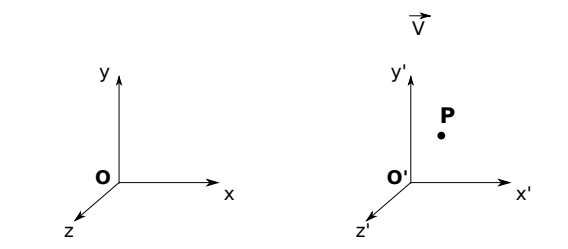
\includegraphics[scale=0.8]{SistemaRiferimento}
        \caption{Sistemi di riferimento}
\end{figure}
Indichiamo con $\vb{X}$ il quadrivettore posizione del punto \textbf{P} rispetto a $\mathbb O$ e $\vb{X^\prime}$ rispetto a $\mathbb O^\prime$, le coordinate di 
$\vb{X^\prime}$ si trovano rispetto alle coordinate misurate in $\mathbb O^\prime$ nel seguente modo : 
\begin{align*}
        \vectorbold{X^\prime} = \vb{\Lambda^{\mu}_{\nu}} \vb{X} 
\end{align*} 
dove $\vb{\Lambda^{\mu}_{nu}}$ rappresenta la matrice della trasformazione di Lorentz lungo asse x data da : 
\begin{align*}
        \vb{\Lambda^{\mu}_{\nu}} = \begin{pmatrix} \gamma & -\gamma\beta & 0 & 0 \\ -\gamma\beta & \gamma & 0 & 0 \\ 0 & 0 & 1 & 0 \\ 0 & 0 & 0 & 1 \end{pmatrix} \tag*{$\beta = \frac{V}{c} \ \ \gamma = \frac{1}{\sqrt{1-\beta^2}}$}\\
\end{align*}

si ottiene :
\begin{align*}
    \systeme*{
    ct^\prime = \gamma ct - \beta\gamma x,
    x^\prime = -\beta\gamma ct + \gamma x,
    y^\prime =y,
    z^\prime =z
}
\end{align*}
Mettere il box in cui spieghi che se beta è piccolo si torna a Galileo e che se si passa da O primo a O cambiano i segni
\newpage
\section{Trasformazione delle velocità}
Per capire bene le trasformazioni delle velocità conviene vedere un esercizio.\\
\textbf{Esercizio : }



\end{document}
